\documentclass[size=a4, parskip=half, titlepage=false, toc=flat, toc=bib, 12pt]{scrartcl}

% ---------------------------------------------------------------------------
%  PAQUETES
% ---------------------------------------------------------------------------

% IDIOMA
\usepackage[utf8]{inputenc}

% MATEMÁTICAS
\usepackage{amsmath}    % Paquete básico de matemáticas
\usepackage{amssymb}	% Fuentes matemáticas
\usepackage{upgreek}
\usepackage{amsthm}     % Teoremas
\usepackage{mathrsfs}   % Fuente para ciertas letras utilizadas en matemáticas

% LISTAS
\usepackage{enumitem}       % Mejores listas
\setlist{leftmargin=.5in}   % Especifica la indentación para las listas.

% Dibujos Tikz
\usepackage{pgf,tikz}
\usepackage{tkz-euclide}
\usetkzobj{all}
\usepackage{mathrsfs}
\usetikzlibrary{arrows, calc,intersections,through,backgrounds}

% Títulos de figuras
\usepackage{capt-of}

% Posición de figuras
\usepackage{float}

% ---------------------------------------------------------------------------
%  RECURSOS
% ---------------------------------------------------------------------------

% Ruta donde buscar gráficos
\graphicspath{{../_assets/}, {_assets/}, {./img/}, {ALGI/img/}, {ALGI/}}

% ---------------------------------------------------------------------------
% ENTORNOS PERSONALIZADOS
% ---------------------------------------------------------------------------

%% DEFINICIONES DE LOS ESTILOS

% Nuevo estilo para definiciones
\newtheoremstyle{definition-style}  % Nombre del estilo
{}                                  % Espacio por encima
{}                                  % Espacio por debajo
{}                                  % Fuente del cuerpo
{}                                  % Identación
{\bfseries\sffamily}                      % Fuente para la cabecera
{.}                                 % Puntuación tras la cabecera
{.5em}                              % Espacio tras la cabecera
{\thmname{#1}\thmnumber{ #2}\thmnote{ (#3)}}  % Especificación de la cabecera

% Nuevo estilo para notas
\newtheoremstyle{remark-style}
{10pt}
{10pt}
{}
{}
{\itshape \sffamily}
{.}
{.5em}
{}

% Nuevo estilo para teoremas y proposiciones
\newtheoremstyle{theorem-style}
{}
{}
{}
{}
{\bfseries \sffamily}
{.}
{.5em}
{\thmname{#1}\thmnumber{ #2}\thmnote{ (#3)}}

% Nuevo estilo para ejemplos
\newtheoremstyle{example-style}
{10pt}
{10pt}
{}
{}
{\bfseries \sffamily}
{}
{.5em}
{\thmname{#1}\thmnumber{ #2.}\thmnote{ #3.}}

% Nuevo estilo para la demostración

\makeatletter
\renewenvironment{proof}[1][\proofname] {\par\pushQED{\qed}\normalfont\topsep6\p@\@plus6\p@\relax\trivlist\item[\hskip\labelsep\itshape\sffamily#1\@addpunct{.}]\ignorespaces}{\popQED\endtrivlist\@endpefalse}
\makeatother

%% ASIGNACIÓN DE LOS ESTILOS

% Teoremas, proposiciones y corolarios
\theoremstyle{theorem-style}
\newtheorem{nth}{Teorema}[section]
\newtheorem{nprop}{Proposición}[section]
\newtheorem{ncor}{Corolario}[section]
\newtheorem{lema}{Lema}[section]

% Definiciones
\theoremstyle{definition-style}
\newtheorem{ndef}{Definición}[section]

% Notas
\theoremstyle{remark-style}
\newtheorem*{nota}{Nota}

% Ejemplos
\theoremstyle{example-style}
\newtheorem{ejemplo}{Ejemplo}[section]

% Ejercicios y solución
\theoremstyle{definition-style}
\newtheorem{ejer}{Ejercicio}[section]

\theoremstyle{remark-style}
\newtheorem*{sol}{Solución}

% ---------------------------------------------------------------------------
% COMANDOS PERSONALIZADOS
% ---------------------------------------------------------------------------

% Números enteros: \ent
\providecommand{\ent}{\mathbb{Z}}

% Números racionales: \rac
\providecommand{\rac}{\mathbb{Q}}

% Números naturales: \nat
\providecommand{\nat}{\mathbb{N}}


% Valor absoluto: \abs{}
\providecommand{\abs}[1]{\lvert#1\rvert}

% Fracción grande: \ddfrac{}{}
\newcommand\ddfrac[2]{\frac{\displaystyle #1}{\displaystyle #2}}

% Texto en negrita en modo matemática: \bm{}
\newcommand{\bm}[1]{\boldsymbol{#1}}

% Línea horizontal.
\newcommand{\horrule}[1]{\rule{\linewidth}{#1}}

% Restricción de una aplicación.
\newcommand\restr[2]{{% we make the whole thing an ordinary symbol
  \left.\kern-\nulldelimiterspace % automatically resize the bar with \right
  #1 % the function
  \vphantom{\big|} % pretend it's a little taller at normal size
  \right|_{#2} % this is the delimiter
  }}

% Imagen de una aplicación.
\DeclareMathOperator*{\img}{img}

% Divisores de un elemento de un anillo
\DeclareMathOperator*{\rdiv}{div}

% Listas ordenadas con números romanos (i), (ii), etc.
\newenvironment{nlist}
{\begin{enumerate}
    \renewcommand\labelenumi{(\emph{\roman{enumi})}}}
  {\end{enumerate}}

% División por casos con llave a la derecha.
\newenvironment{rcases}
{\left.\begin{aligned}}
    {\end{aligned}\right\rbrace}


% ---------------------------------------------------------------------------
%  COLORES
% ---------------------------------------------------------------------------

\usepackage{xcolor}     % Permite definir y utilizar colores

\definecolor{50}{HTML}{FFEBEE}
\definecolor{300}{HTML}{E57373}
\definecolor{500}{HTML}{F44336}
\definecolor{700}{HTML}{D32F2F}
\definecolor{900}{HTML}{B71C1C}


\setuptoc{toc}{leveldown}

% Ajuste de las líneas y párrafos
\linespread{1.2}
\setlength{\parindent}{0pt}
\setlength{\parskip}{12pt}

% Español
\usepackage[spanish, es-tabla]{babel}

% Matemáticas
\usepackage{amsmath}
\usepackage{amsthm}

% Links
%\usepackage{hyperref}

% Fuentes
\usepackage{newpxtext,newpxmath}
\usepackage[scale=.9]{FiraMono}
\usepackage{FiraSans}
\usepackage[T1]{fontenc}

\defaultfontfeatures{Ligatures=TeX,Numbers=Lining}
\usepackage[activate={true,nocompatibility},final,tracking=true,factor=1100,stretch=10,shrink=10]{microtype}
\SetTracking{encoding={*}, shape=sc}{0}

\usepackage{graphicx}
\usepackage{float}

% Mejores tablas
\usepackage{booktabs}

\usepackage{adjustbox}

% COLORES

\usepackage{xcolor}

\definecolor{verde}{HTML}{007D51}
\definecolor{esmeralda}{HTML}{045D56}
\definecolor{salmon}{HTML}{FF6859}
\definecolor{amarillo}{HTML}{FFAC12}
\definecolor{morado}{HTML}{A932FF}
\definecolor{azul}{HTML}{0082FB}
\definecolor{error}{HTML}{b00020}

% ENTORNOS
\usepackage[skins, listings, theorems]{tcolorbox}

\newtcolorbox{recuerda}{
  enhanced,
%  sharp corners,
  frame hidden,
  colback=black!10,
	lefttitle=0pt,
  coltitle=black,
  fonttitle=\bfseries\sffamily\scshape,
  titlerule=0.8mm,
  titlerule style=black,
  title=\raisebox{-0.6ex}{\small RECUERDA}
}

\newtcolorbox{nota}{
  enhanced,
%  sharp corners,
  frame hidden,
  colback=black!10,
	lefttitle=0pt,
  coltitle=black,
  fonttitle=\bfseries\sffamily\scshape,
  titlerule=0.8mm,
  titlerule style=black,
  title=\raisebox{-0.6ex}{\small NOTA}
}

\newtcolorbox{error}{
  enhanced,
%  sharp corners,
  frame hidden,
  colback=error!10,
	lefttitle=0pt,
  coltitle=error,
  fonttitle=\bfseries\sffamily\scshape,
  titlerule=0.8mm,
  titlerule style=error,
  title=\raisebox{-0.6ex}{\small ERROR}
}

\newtcblisting{shell}{
  enhanced,
  colback=black!10,
  colupper=black,
  frame hidden,
  opacityback=0,
  coltitle=black,
  fonttitle=\bfseries\sffamily\scshape,
  %titlerule=0.8mm,
  %titlerule style=black,
  %title=Consola,
  listing only,
  listing options={
    style=tcblatex,
    language=sh,
    breaklines=true,
    postbreak=\mbox{\textcolor{black}{$\hookrightarrow$}\space},
    emph={jmml@UbuntuServer, jmml@CentOS},
    emphstyle={\bfseries},
  },
}

\newtcbtheorem[number within=section]{teor}{\small TEOREMA}{
  enhanced,
  sharp corners,
  frame hidden,
  colback=white,
  coltitle=black,
  fonttitle=\bfseries\sffamily,
  %separator sign=\raisebox{-0.65ex}{\Large\MI\symbol{58828}},
  description font=\itshape
}{teor}

\newtcbtheorem[number within=section]{prop}{\small PROPOSICIÓN}{
  enhanced,
  sharp corners,
  frame hidden,
  colback=white,
  coltitle=black,
  fonttitle=\bfseries\sffamily,
  %separator sign=\raisebox{-0.65ex}{\Large\MI\symbol{58828}},
  description font=\itshape
}{prop}

\newtcbtheorem[number within=section]{cor}{\small COROLARIO}{
  enhanced,
  sharp corners,
  frame hidden,
  colback=white,
  coltitle=black,
  fonttitle=\bfseries\sffamily,
  %separator sign=\raisebox{-0.65ex}{\Large\MI\symbol{58828}},
  description font=\itshape
}{cor}

\newtcbtheorem[number within=section]{defi}{\small DEFINICIÓN}{
  enhanced,
  sharp corners,
  frame hidden,
  colback=white,
  coltitle=black,
  fonttitle=\bfseries\sffamily,
  %separator sign=\raisebox{-0.65ex}{\Large\MI\symbol{58828}},
  description font=\itshape
}{defi}

\newtcbtheorem{ejer}{\small EJERCICIO}{
  enhanced,
  sharp corners,
  frame hidden,
  left=0mm,
  right=0mm,
  colback=white,
  coltitle=black,
  fonttitle=\bfseries\sffamily,
  %separator sign=\raisebox{-0.65ex}{\Large\MI\symbol{58828}},
  description font=\itshape,
  nameref/.style={},
}{ejer}

% CÓDIGO
\usepackage{listings}

% CABECERAS
\pagestyle{headings}
\setkomafont{pageheadfoot}{\normalfont\normalcolor\sffamily\small}
\setkomafont{pagenumber}{\normalfont\sffamily}

% ALGORITMOS
\usepackage[vlined,linesnumbered]{algorithm2e}

% Formato de los pies de figura
\setkomafont{captionlabel}{\scshape}
\SetAlCapFnt{\normalfont\scshape}
\SetAlgorithmName{Algoritmo}{Algoritmo}{Lista de algoritmos}

% BIBLIOGRAFÍA
%\usepackage[sorting=none]{biblatex}
%\addbibresource{bibliografia.bib}

\begin{document}

\renewcommand{\proofname}{\normalfont\sffamily\bfseries\small DEMOSTRACIÓN}

\title{Método de ranking en el diseño de un sistema de acceso a la información}
\subject{Trabajo fin de grado}
\author{Johanna Capote Robayna\\
    Doble Grado en Ingeniería Informática y Matemáticas}
\date{}
\publishers{\vspace{2cm}
\includegraphics[height=2.5cm]{UGR}\vspace{1cm}}
\maketitle

\newpage

\tableofcontents
\newpage

\section{Introducción}
Fue en la década de los 80, cuando Internet empieza a darse a conocer con unas primeras páginas web de estilo muy básico y sencillo que tardaban mucho en cargarse. Con el transcurso del tiempo la Red fue creciendo a pasos agigantados almacenando un gran volumen de información lo que provocó  un sinfín de procesos y cambios en las formas de gestionarla, y es en ese contexto donde surgen los buscadores para dar respuesta a la necesidad de clasificar y gestionar gran cantidad de información lo más rápido posible.

Un buscador o motor de búsqueda es un sistema de recuperación de información, donde el usuario introduce una serie de términos o palabras clave y el buscador le devuelve una lista de resultados ordenados bajo una serie de criterios. WebCrawler, Lycos, AltaVista o Yahoo entre otros, son los primeros buscadores de la Historia que funcionaban de una forma muy similar, rastreaban la Red y clasificaban las páginas en función de las veces que contenían las palabras clave introducidas. Eran los más utilizados en esa época hasta que en 1998 son desbancados por Google, el mayor motor de búsqueda de todos los tiempos,  que consigue imponerse al resto de buscadores gracias a un nuevo algoritmo de búsqueda (PageRank), capaz de ordenar una gran cantidad de información en poco tiempo.

PageRank, es un algoritmo basado en el Álgebra lineal, Teoría de Grafos y Probabilidad, fue diseñado por Sergey Brin y Lawrence Page, el primero graduado en Matemáticas y el segundo en Informática y ambos estudiantes de doctorado de Informática de la Universidad de Standford. La pregunta que buscaban resolver era clara ``?`en qué orden mostrar los resultados de la búsqueda?''. En 1997 cuando Brin y Page empezaron a trabajar en el diseño del algoritmo se plantearon como objetivo principal que en el gran número de los casos, al menos una de las primeras páginas que se muestran como resultado contenga información útil para el usuario. Hay que tener en cuenta que en esta época Internet no era tan grande como ahora, habían censadas en torno a 100 millones de páginas web y los buscadores más famosos de la época eran capaces de atender 20 millones de consultas al día, mientras que hoy en día Google es capaz de atender a 200 millones de consultas diarias. Pasaremos a explicar como el algoritmo de PageRank es capaz de ordenar estas millones de páginas web en tan poco tiempo.

\section{El modelo}

\subsection{Introducción al modelo}
Lo primero que hace Google, incluso antes de que el usuario realice la búsqueda es organizar el contenido de Internet ayudándose de un índice. Este índice se va actualizando y va añadiendo páginas nuevas y modificando la información de las páginas ya añadidas en un proceso llamado ``rastreo'', en el cual adquiere información de esas páginas incluyendo los enlaces hacia otra páginas. El índice se ordena con el algoritmo de \textbf{PageRank}, el cual se explicará a continuación, que ordena la lista asignando un PageRank más alto a las páginas que calificará de ``más interesantes'' y un PageRank bajo a las páginas ``menos interesantes''.

Una vez que el usuario introduce su búsqueda esta pasa por varias fases:
\begin{itemize}
\item Análisis de las palabras del usuario. En esta fase se busca entender el significado de la búsqueda, para ello se analiza las palabras usadas y se interpreta lo que el usuario quiere decir con ellas. Este proceso incluye varios pasos como \textbf{interpretar los errores de ortografía} o entender el significado que el usuario le está dando a una palabra con varias acepciones ayudándose de un \textbf{sistema de sinónimos}. Otro aspecto importante de esta fase es el \textbf{algoritmo de novedades}, el cual deduce que en ciertas búsquedas debe mostrar la información más actual, como por ejemplo si el usuario busca ``horóscopo'' o ``resultados del fútbol club Granada'' se está interesando por las últimas publicaciones.
\item Búsqueda de coincidencias. En esta fase se busca entre las páginas del índice aquellas con información coincidente con la búsqueda. Se analiza la frecuencia con la que aparecen las palabras introducidas en las páginas web candidatas y su localización; es decir, si aparecen en el título, encabezamientos o en el cuerpo del texto. Además existen otros algoritmos que analizan si las páginas candidatas pueden resultar interesantes para el usuario, ya que si por ejemplo el usuario busca ``pájaros'' lo más probable es que no quiera encontrar una página con poca información relevante sobre el tema pero en la que se repite muchas veces la palabra ``pájaro''.
\item Mejora del posicionamiento de las páginas útiles. Una vez obtenidas las páginas web con información potencialmente válidas se pasa a clasificar su utilidad con el objetivo de mostrar primero las páginas más útiles para el usuario. En esta fase se analizan varios factores como el número de veces que aparece el término buscado en la página, la fecha de publicación y la calidad de experiencia del usuario en la página. Además se descartan aquellos sitios web con contenido fraudulento o \textit{spam} y se potencia las páginas que en consultas similares hayan sido fiables.
\item Devolver los mejores resultados. En esta parte se busca la diversidad de respuestas. Antes de mostrar el resultado de la búsqueda se analiza el resultado en conjunto, se evalúa si hay muchas páginas centradas en la misma interpretación de la búsqueda o si solo existe un tema en los resultados.
\item Análisis del contexto. Esta fase no se realiza siempre, en ella se busca ``personalizar'' la búsqueda con datos como la ubicación o historial de búsqueda. Con ello se consigue reducir la búsqueda a su entorno, por ejemplo si el usuario es español y busca ``baloncesto'' le saldrá antes información sobre el baloncesto en España que sobre el de otros países o si el usuario busca ``conciertos cerca de mi'' aparecerán los conciertos más cercanos a su residencia. Además mediante el historial de búsqueda personal el buscador consigue mejorar la interpretación de la búsqueda, por ejemplo si el usuario ha buscado anteriormente ``Granada vs Osasuna'' y más adelante busca ``Granada'' puede considerar que el usuario se refiere al equipo de fútbol y no a la ciudad.
\end{itemize}

\subsection{Modelo matemático}

El algoritmo de PageRank utilizado para ordenar las páginas web tiene una base matemática basado en el álgebra lineal, veamos como se transforma el problema de ordenar las páginas web según su interés en un problema clásico de autovalores y autovectores.

En primer lugar, vamos a definir el marco donde nos encontramos. Nuestro problema actual es establecer un criterio para ordenar las páginas de la red. Si llamamos $P_1, \dots, P_n$ a cada una de las páginas, siendo $n$ un número natural ($n \in \mathbb{N}$), definimos entonces la importancia $x_i$  de la página $P_i$ como un número real entre $0$ y $1$.

Esta importancia la utilizaremos para elegir que páginas web son las primeras que mostramos en el buscador, ordenándolas de mayor  a menor valor de importancia.
Para calcular este número nos basamos en la información que podemos extraer de la red (sitios, contenido, enlaces de una página web a otra, etc).

En el primer modelo nos quedamos solo con los enlaces entre páginas web. Estos enlaces los podemos representar mediante un grafo dirigido (G), en la cual representamos cada $P_i$ como un nodo del grafo y por cada enlace de una página $P_i$ a $P_j$ añadimos una arista de $P_j$ a $P_i$ indicando el final con una punta de flecha, como se indica en la imagen.

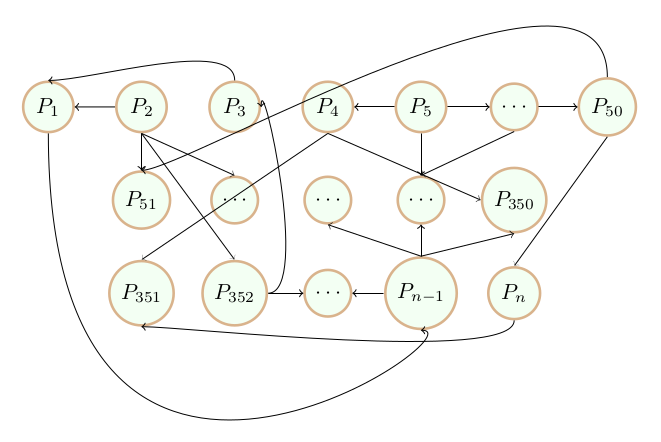
\includegraphics[width=1.0\textwidth]{./img/grafoini}

Esta información la podemos reflejar en una matriz M de dimensión $nxn$. Tanto en las filas como en las columnas representamos las $n$ páginas y por cada enlace entre una página $j$ a otra página $i$, escribimos un $1$ en la entrada de la
matriz $m_{i,j}$ y en el caso de que no haya enlace escribimos un $0$.

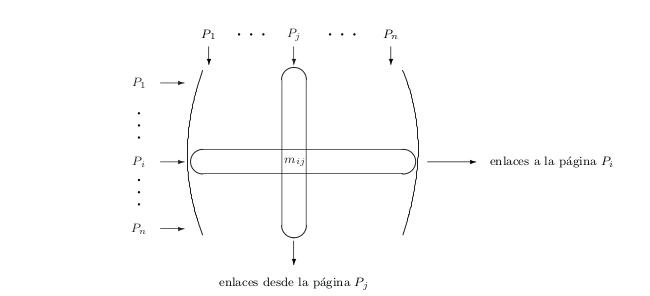
\includegraphics[width=1.0\textwidth]{./img/matriz}

Por lo tanto en la columna $j$ estarán los enlaces que salen de la página $P_j$ hacia otras páginas
mientras que en la fila $i$ estarán representados los enlaces a la página $P_i$. De lo que se deduce que esta matriz
no es simétrica ya que una página puede estar citada por otra y ella no citar a ninguna.

En una primera aproximación de querer ordenar las páginas web por ``importancia'' o ``relevancia'' podemos
pensar que la página a la que le lleguen más enlaces (fila con mayor número de $1$) es la que debería
mostrarse primero en el \textit{ranking}. Es decir si $x_j$ es la importancia de $P_j$, esta es proporcional
al número de páginas desde las que hay enlaces a $P_j$.

Sin embargo, la realidad es que el número de enlaces a una cierta página no representa del todo su importancia,
ya que no es lo mismo que esta esté citada por una página cualquiera a que esté citada desde \verb|www.facebook.com| o
\verb|www.apple.com|. Estos dos últimos enlaces deberían ponderar más en importancia que otras citas de
otras páginas web menos relevantes. Por lo que para asignar importancia a una página web, deberemos tener
en cuenta tanto si es una \textbf{página muy citada} como si es una \textbf{página poco citada, pero de sitio ``relevantes''}.

Nos damos cuenta de la que importancia de la página citadora también es importante, por lo que en una segunda aproximación pasamos a decidir que la importancia $x_j$ de una página $P_j$ es proporcional a la suma de las importancias de las páginas que enlazan con $P_j$. El cambio reside en que en la primera aproximación del modelo la importancia de $P_i$ era proporcional al número de páginas que enlazan con $P_i$, mientras que en esta segunda aproximación la importancia de $P_i$ es proporcional a la suma de las importancias de las páginas que enlazan con $P_i$.

Supongamos, por ejemplo, que la página $P_1$ es citada desde las páginas $P_{200}$ y $P_{n}$ ,
 que $P_2$ se cita desde $P_1$ , $P_{50}$ , $P_{200}$ y $P_n$ , mientas que en la última página $P_n$ hay enlaces desde $P_1$ , $P_2$ , $P_{50}$ , $P_{200}$ y $P_{n-1}$. En nuestra asignación anterior, $x_1, \dots , x_n$ deberían
 cumplir entonces que:
 $$ x_1 = K (x_{200} + x_n) $$
 $$ x_2 = K (x_{50} + x_{200} + x_{n-1}) $$
 $$ \vdots $$
 $$x_n = K (x_1 + x_2 + x_{50} + x_{200} + x_{n-1}) $$

donde $K$ es una constante de proporcionalidad. Si nos fijamos, hemos construido un sistema de ecuaciones
donde las soluciones son los posibles valores de $x_1, \dots , x_n$. Este sistema de ecuaciones
lo podemos escribir en términos matriciales:

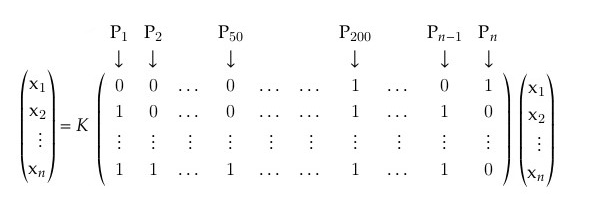
\includegraphics[width=1.0\textwidth]{./img/matrizejemplo}

Si llamamos $X$ al vector de importacias $(x_1 \dots x_n)$, llamamos $\lambda = \frac{1}{K}$ y llamamos
$M$ a la matriz de dimensiones $n x n$ del sistema (matriz asociada al grafo). Nos encontramos
con un problema de autovalores y autovectores:
$$Mx = \lambda x $$

A este vector $x$ le exigimos que sea no negativo, es decir $x \leq 0$ ya que representa la importancia
de una página web y también buscamos que sea único ya que como nuestro objetivo final es establecer un
\textit{ranking} de haber más de uno habría que diseñar otro proceso de selección.
El hecho de que el vector $x$ sea no negativo convierte a la matriz $M$ en no negativa ($M \leq 0$), ya que sus filas
están los valores $x_1, \dots , x_n$.

\subsection{Justificación matemática}

Hemos conseguido ver que resolver el problema de ordenar las páginas web por importancia equivale a resolver un problema de autovalores y autovectores, por lo que solo nos falta ver si ese $\lambda$ que estamos buscando existe.

En primer lugar, vamos a definir el marco donde nos encontramos. Al igual que antes llamamos $P_1, \dots, P_n$ a cada una de las páginas, siendo $n$ un número natural ($n \in \mathbb{N}$), definimos entonces la importancia $x_i$  de la página $P_i$ como un número real entre $0$ y $1$.

Llamamos $G$ al grafo que representa los enlaces entre páginas web, en el cual representamos cada $P_i$ como un nodo del grafo y por cada enlace de una página $P_i$ a $P_j$ añadimos una arista de $P_j$ a $P_i$. Por último llamamos $M \in  M_n(\mathbb{R})$ a la matriz de adyacencia del grafo, es decir aquella matriz en la que se representan tanto en las filas como en la columnas los nodos y por cada enlace entre $P_i$ y $P_j$ sumamos 1 en la celda M[j,i].

\begin{ndef}[Matriz irreducible]
Se dice que una matriz $A \in M_n(\mathbb{R})$ es irreducible cuando cumple alguna de las siguientes:
\begin{enumerate}
\item No existe ninguna permutación (de filas y columnas) que transforma $A$ en una matriz del tipo:
\begin{center}
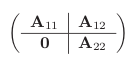
\includegraphics[width=0.2\textwidth]{./img/mcuadrada}
\end{center}
donde $A_{11}$ y $A_{22}$ son matrices cuadradas.
\item La matriz $(I + A)^{n - 1}$, donde $I$ es la identidad $n x n$, tiene todas sus entradas positivas.
\item Si $A$ es la matriz de adyacencia de un grafo, entonces el grafo está fuertemente conectado.
\end{enumerate}
\end{ndef}

\textbf{?`?`Grafo fuertemente conectado o fuertemente conexo??}

Por lo tanto por definición, nuestra matriz $M$ sería irreducible si el grafo $G$ estuviera fuertemente conectado. Por otro lado el teorema de Perron demostraría la existencia y unicidad de nuestro vector solución $x$, sin embargo nuestra matriz $M$ puede tener entradas nulas por lo que no nos serviría el resultado.

\begin{nth}[Perron, 1907]
Sea $A$ una matriz cuadrada ($A \in M_n(\mathbb{R})$) con entradas positivas, $A > 0$. Entonces:
\begin{enumerate}
\item Existe un autovalor (simple) \lamda > 0 tal que $Av = \lambda v$ donde el autovector es $v > 0$.
\item Este autovalor es mayor, en módulo, que todos los demás autovalores.
\item Cualquier otro autovector positivo de $A$ es un múltiplo de $v$.
\end{enumerate}
\end{nth}

Unos años después Frobenius publica un resultado similar para las matrices de entradas no negativas e irreducibles. Para aplicar este teorema solo faltaría demostrar que nuestra matriz $M$ es irreducible.

\begin{nth}[Frobenius, 1908-1912]
Sea $A $ una matriz cuadrada con entradas no negativas ($A \leq 0$). Si $A$ es irreducible, entonces:
\begin{enumerate}
\item Existe un autovalor (simple) $\lambda > 0$ tal que $A v = \lambda v$, donde el autovector es
$v > 0$. Además, $\lambda \leq |\mu|$, para cualquier otro autovalor $\mu$ de $A$.
\item Cualquier autovector $\leq 0$ es múltiplo de $v$.
\item Si hay $k$ autovalores de módulo máximo, entonces son las soluciones de $x^k - \lambda^k = 0$.
\end{enumerate}
\end{nth}

\newpage

\section{Pseudocódigo}

\begin{algorithm}[H]
  \KwData{Matriz de enlaces (m); Número de interaciones (num\_iter); Factor (d)}
  \KwResult{Vector de pesos del PageRank (v)}

  N = M[0].size()\;
  v = random(N, 1)\;
  v = v / max(v)\;
  \For{i $\in$ num\_iter}{
    v = d * m * v + (1 - d)/ N
  }
  \Return v

\end{algorithm}
M_{i,j} =
\begin{bmatrix}
0 & 0 & 0 & 0 & 1 \\
0.5 & 0 & 0 & 0 & 0 \\
0.5 & 0 & 0 & 0 & 0 \\
0 & 1 & 1 & 0 & 0 \\
0 & 0 & 0 & 1 & 0
\end{bmatrix}

donde se representa el enlace de i a j.


\section{Ejemplo}
Para ilustrar mejor el algoritmo, veamos un ejemplo con 5 nodos referenciados de la siguiente forma:

\begin{figure}[H]
\centering
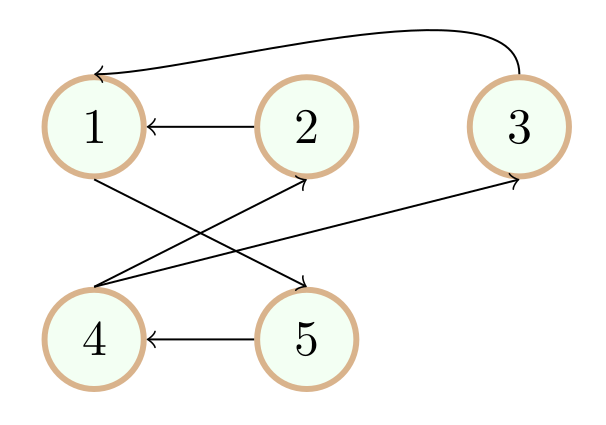
\includegraphics[scale=0.5]{./img/grafoejemplo}
\end{figure}
Donde el inicio de la flecha indica el autor que ha sido referenciado y la punta de la flecha indica
que ese autor ha citado el autor del que sale la flecha. Por lo tanto en el algoritmo debería de salir
el autor número $4$ el primero ya que de él salen dos flechas, mientras que de los demás autores salen
como máximo una flecha. Los resultados obtenidos son:

\begin{verbatim}
[[0.2385439 ]
 [0.13138118]
 [0.13138118]
 [0.25334798]
 [0.24534576]]
\end{verbatim}

Donde vemos que el peso mayor se encuentra en el puesto número 4, es decir el cuarto autor sería el
primero en salir en el ranking. Observamos que de los demás nodos siempre sale una sola flecha, sin
embargo el segundo y tercer puesto del ranking es el autor número $5$ y el número $1$. Esto es debido
a que el autor referencia tanto al nodo $2$ como al nodo $3$ por lo que al normalizar estas
referencias el valor de la referencia se divide a la mitad, si le pusiéramos pesos a las flechas,
estas dos flechas que llegan al nodo $1$ valdrían $0.5$. Esto tiene sentido ya que lo que se premia
en este algoritmo es que un articulo este citado por varios autores y no que el mismo autor cite todos
los autores. Por lo tanto si en un artículo se cita solo un autor, el peso de la flecha será uno
mientras que si un autor referencia $N$ autores cada flecha de referencia pesará $\frac{1}{N}$.

\section{Sistema basado en la información}
Un sistema de acceso a la información es un sistema dotado de un conjunto de técnicas para buscar, categorizar, modificar y acceder a la información que se encuentra en un sistema: base de datos, bibliotecas, archivos o internet.

\section{Base de datos}

Para realizar un estudio de \textit{pagerank} se ha utilizado la base de datos \textbf{PMSC-UGR} con
$26759991$ artículos. Esta base de datos basada en articulos científicos de MEDLINE/PubMed  pero
también utilizando SCopus herramienta de Elsevier. En PSMC-UGR se ha hecho el esfuerzo de
quitar las ambigüedades de los nombres de autores, para ello se ha establecido el ORCID, un número
que identifica a cada autor de manera univoca. Cada archivo esta estructurado de la siguiente forma:
\begin{itemize}
\item \textit{PubMedID}. Es un identificador único del articulo proporcionado por PubMed.
\item \textit{Journal}. Es el nombre de la revista donde el artículo ha sido publicado.
\item \textit{ArticleTitle}. Es el título completo del artículo en inglés.
\item \textit{Abstract}. Resumen del artículo.
\item \textit{AuthorList}. Contiene información sobre los autores del artículo. Por cada uno podemos encontrar:
\begin{itemize}
\item \textit{LastName}. Contiene el apellido o el nombre único utilizado.
\item \textit{ForeName}. Contiene el resto del nombre.
\item \textit{Identifier}. Es un identificador único asociado con el nombre (ORCID).
\end{itemize}
\item \textit{MeshHeadingList}. Es un vocabulario controlado por NLM, encabezados de temas médicos (Mesh). Se utiliza para caracterizar el contenido del artículo, utilizando descriptores de ese tesauro.
\item \textit{KeywordList}. Contiene términos controlados en palabras clave que también describen el contenido del artículo.
\end{itemize}

A estos datos se añaden las citas, el $66.78 \%$ de los artículos tienen alguna cita. La media de citas por artículo es de 7 y el total de citas es $3593931$. El numero de citas por articulo sigue una típica distribución \textit{ley de potencia}, donde pocos artículos tienen muchas citas y muchos artículos tienen pocas citas. Por ejemplo, hay $116365$ artículos que tienen solo una cita y hay un artículo que tiene 713 citas.

\textbf{?`?` Esto se refiere a citas y referencias o las referencias van a parte??}
%printbibliography

\end{document}
